%%%%%%%%%%%%%%%%%%%%%%%%%%%%%%%%%%%%%%%%%%%%%%%%%%
\documentclass[12pt]{article}
\usepackage{epsfig,verbatim}
\usepackage{color}
%\pagestyle{headings}
\textheight 8.5 in
\textwidth 6.5 in
\topmargin -0.35 in
%\topmargin -0.10 in
\oddsidemargin -0.1 in
\renewcommand{\topfraction}{1}
\renewcommand{\bottomfraction}{1}
\renewcommand{\textfraction}{0}
\renewcommand{\floatpagefraction}{0.90}
\makeatletter
\def\singlespace{\def\baselinestretch{1}\@normalsize}
\def\endsinglespace{}
\newtheorem{lemma}{Lemma}%[section]
\newtheorem{theorem}{Theorem}%[section]
\newtheorem{remark}{Remark}
\newtheorem{example}{Example}%[section]
\newtheorem{corollary}{Corollary}%[section]
\@addtoreset{equation}{section}
\renewcommand{\theequation}{\thesection.\arabic{equation}}
\renewcommand{\thefootnote}{\fnsymbol{footnote}}
\renewcommand{\hat}{\widehat}
\def\singlespace{\def\baselinestretch{1}\@normalsize}
\def\endsinglespace{}
\makeatother
\def\c{\centerline}
\newcommand{\by}{\mbox{\bf y}}
\newcommand{\bX}{\mbox{\bf X}}
\newcommand{\bZ}{\mbox{\bf Z}}
\newcommand{\bz}{\mbox{\bf z}}
\newcommand{\bx}{\mbox{\bf x}}
\newcommand{\bV}{\mbox{\bf V}}
\newcommand{\ba}{\mbox{\bf a}}
\newcommand{\bb}{\mbox{\bf b}}
\newcommand{\pl}{p_{\lambda}}
\newcommand{\bbeta}{\mbox{\boldmath$\beta$}}
\newcommand{\bga}{\mbox{\boldmath$\gamma$}}
\newcommand{\balpha}{\mbox{\boldmath$\alpha$}}
\newcommand{\bpsi}{\mbox{\boldmath$\psi$}}


\newcommand{\btheta}{\mbox{\boldmath$\theta$}}
\newcommand{\hbeta}{\hat{\beta}}
\newcommand{\hbbeta}{\hat{\bbeta}}
\newcommand{\halpha}{\hat{\alpha}}
\newcommand{\htheta}{\hat{\theta}}
\newcommand{\hbtheta}{\hat{\btheta}}
\newcommand{\bW}{\mbox{\bf W}}
\newcommand{\bvar}{\mbox{\boldmath$\varepsilon$}}

% =================== THE SELF-DEFINED COMMANDS =============================
\font\larges=cmbx8 scaled 1500
\def\newpage{\vfill\eject}
 \def\wh{\widehat}
 \def\Var{\mbox{Var}}
\def\MSE{\mbox{MSE}}
 \def\andd{\mbox{and}}
 \def\logit{\mbox{logit}}
\def\new{\mbox{new}}
\def\say{\mbox{(say)}} \def\wt{\widetilde}
\def\today{\ifcase\month\or
  January\or February\or March\or April\or May\or June\or
  July\or August\or September\or October\or November\or December\fi
  \space\number\day, \number\year}
\def\Cov{\mbox{Cov}}  \def\C{\mbox{const.}\quad} \def\no{\noindent}
\def\proof{{\noindent\underbar{\bf Proof}\quad}}
\def\Lemma#1{{\noindent\underbar{\bf Lemma #1}\quad}}
\def\Theorem#1{{\noindent\underbar{\bf Theorem #1}\quad}}
\def\Remark#1{{\noindent\underbar{\bf Remark #1}\quad}}
\def\endp{{\vrule width 5pt height 5pt\par}}
\def\d{\quad{\buildrel  {\cal D}\over\longrightarrow}\quad}
\newdimen\biblioindent    \biblioindent=30pt
\def\bibentry{\hangindent=\biblioindent}
\def\wh{\widehat}
\font\smallfont=cmr8 at 7truept
\def\MLE{\mbox{\smallfont{MLE}}}
\def\U{\mbox{\smallfont{U}}}
\def\sgn{\mbox{sgn}}

\def\bH{{\bf H}}
\def\bU{{\bf U}}
\def\bu{{\bf u}}
\def\bV{{\bf V}}
\def\bI{{\bf I}}
\def\bv{{\bf v}}
\def\bY{{\bf Y}}
\def\diag{\mbox{diag}}
\def\supp{\mbox{supp}}
\def\MSE{\mbox{MSE}}
\def\MMSE{\mbox{MMSE}}
\def\SMSE{\mbox{SMSE}}
\def\cov{\mbox{cov}}
\def\gcv{\mbox{GCV}}
\def\tr{\mbox{tr}}
\def\argmin{\mbox{argmin}}
\def\var{\varepsilon}
\def\la{\lambda}
\def\si{\sigma}
\def\rss{(\bY-\bX\bbeta)^T(\bY-\bX\bbeta)}
\newcommand{\be}{\begin{equation}}
\newcommand{\ee}{\end{equation}}
\newcommand{\beq}{\begin{equation}}
\newcommand{\eeq}{\end{equation}}
\newcommand{\beqn}{\begin{eqnarray}}
\newcommand{\eeqn}{\end{eqnarray}}
\newcommand{\beqnn}{\begin{eqnarray*}}
\newcommand{\eeqnn}{\end{eqnarray*}}

\newtheorem{thm}{Theorem}[section]
\newtheorem{lem}{Lemma}[section]
\newtheorem{rem}{Remark}[section]
\newtheorem{cor}{Corollary}[section]
\newtheorem{exam}{Example}[section]
\newtheorem{ass}{Assumption}[section]
\newtheorem{prop}{Proposition}[section]

\def\S{{\bf A}}
\def\s{{\bf a}}
\def\eps{\varepsilon}

\newcommand{\pln}{p_{\lambda_n}}
\newcommand{\etal}{{\it et al }}
\newcommand{\eg}{{\it e.g. }}
\newcommand{\what}{\widehat}

% ================END OF THE SELF-DEFINED COMMANDS =====================

\begin{document}
\renewcommand{\baselinestretch}{1.5}

\title{Linear Classification Methods and QDA}

\author{\sc John Ensley and Songshan Yang}

\date{\today}
\maketitle
\section{Introduction of the data set}

In this project, we applied the linear classification methods and QDA to a breast cancer data set. This breast cancer database was obtained from the University of Wisconsin Hospitals, Madison from Dr. William H. Wolberg.
There are $699$ subjects with tumors in the data set. All of the tumors are classified as one of two different classes --- either ``Benign'' or ``Malignant''. There are $9$ features measured for each tumor, including clump thickness, uniformity of cell size, uniformity of cell shape, marginal adhesion, single epithelial cell Size, bare nuclei, bland chromatin, normal nucleoli, and mitoses. All of them range in value from $1$ to $10$.



\section{LDA, QDA and Logistic Regression}
In the first step, we applied LDA, QDA and logistic regression to the whole data set to examine their classification error rate. We found that there are only $16$ subjects that have missing data and we deleted these subjects, since the results will not be affected because of the large sample size. 

There are $458$ subjects belonging to Benign and $241$ subjects belonging to Malignant, so the prior probabilities are $\pi_1=0.65$ and $\pi_2=0.35$ for benign and malignant, respectively. For LDA, we compute the means of the class ``Benign'' and ``Malignant'' and the covariance matrix of the $9$ features. Then we classify the subjects according to the maximum of their discriminant functions. For QDA, the process is similar to that of LDA, but we instead compute the covariance matrix for each class and then classify the subjects. For logistic regression, we use the Newton-Raphson algorithm to finish the optimization problem.   

We randomly selected approximately half of the data set to use as training data, and used the rest for testing. The classification results are summarized in Table \ref{tab1}.


\begin{table}[htbp]
\begin{center}
\caption{\label{tab1} Classification Error Rate of LDA, QDA and Logistic Regression}
\begin{tabular}{c|ccc}
				\hline
Method&LDA &QDA &Logistic Regression \\
				\hline
Error Rate &0.0395 &0.0401 &0.0307  \\
				\hline
\end{tabular}
\end{center}
\end{table}
From Table \ref{tab1}, we can see that LDA and QDA have similar classification error rates and logistic regression outperforms the LDA and QDA in the classification.


\section{PCA on LDA, QDA and Logistic Regression}
In this section, we examined the effect of dimension reduction on classification. We first standardized the design matrix and did eigen-decomposition of the covariance matrix of the standardized design matrix. The ratio of how much each principle component explains the total variance is summarized in Table \ref{tab2}.
\begin{table}[htbp]
	\begin{center}
	
		\caption{\label{tab2} Classification Error Rate of LDA, QDA and Logistic Regression}
		\begin{tabular}{c|cccccccccc}
			\hline
Ratio &0.655& 0.086& 0.060& 0.051& 0.042& 0.034& 0.033& 0.029& 0.010 \\
			\hline
	\end{tabular}
	\end{center}
\end{table}
We decided to use the first two components which account for about $74$\% of the total variance. Then the design matrix only has two columns. By repeating the process described in section 2, the classification error rates are summarized in Table \ref{tab3}.
\begin{table}[htbp]
	\begin{center}
		\caption{\label{tab3} Classification Error Rate of LDA, QDA and Logistic Regression}
		\begin{tabular}{c|ccc}
			\hline
			Method&LDA &QDA &Logistic Regression \\
			\hline
			Error Rate &0.0395 &0.0337 &0.0307  \\
			\hline
		\end{tabular}
	\end{center}
\end{table}
Comparing Table \ref{tab3} and Table \ref{tab1}, we can see that PCA only improves the performance of QDA, and it does not have an effect on LDA or logistic regression. See Figure~\ref{fig:lda} for the decision boundary resulting from LDA with dimension reduction.

\begin{figure}[tb]
	\centering
	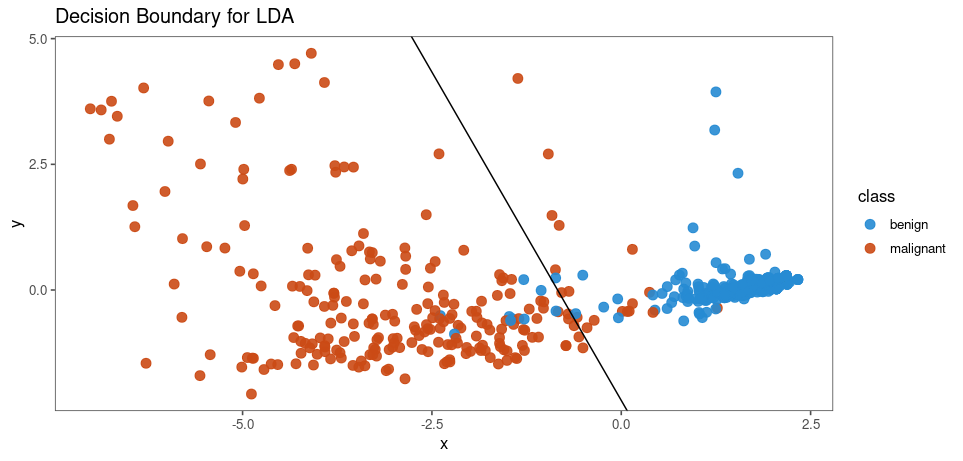
\includegraphics[width=0.8\textwidth]{lda.png}
	\caption{Decision boundary for LDA after reducing to two dimensions using PCA.}
	\label{fig:lda}
\end{figure}

\section{Classification Using Cross-validation}
In this section we explored the classification accuracy using cross-validation. We use 2, 4, 6, 8 and 10-fold cross-validation to examine the effect of cross-validation on the classification method and also the number of folds on the error rate. The results are summarized in Table \ref{tab4}. All the results are based on 100 simulations. 
\begin{table}[htbp]
	\begin{center}
		\caption{\label{tab4} Classification Error Rate of LDA, QDA and Logistic Regression using cross-validation}
		\begin{tabular}{c|c|ccc}
			\hline
			&&LDA &QDA &Logistic Regression \\
            \hline
            Error Rate& 2&0.0468 &0.0454 &0.0410  \\ 
           \hline
	       &4 &0.0395 &0.0512 &0.0322  \\ 
		     \hline
		  &6 &0.0395 &0.0468 &0.0307  \\
		    \hline
		&8 &0.0395 &0.0483 &0.0307  \\
			\hline
		&10 &0.0395 &0.0483 &0.0351  \\
			\hline
		\end{tabular}
	\end{center}
\end{table}

From Table \ref{tab4}, we can see that the performances of LDA, QDA and logistic regression are not changed too much when we use cross-validation and the number of folds does not affect the performances significantly.


We then evaluate the classification method with reduced dimension using cross-validation. We again use 2, 4, 6, 8 and 10-fold cross-validation to examine the effect of cross-validation on the classification method and also the number of folds on the error rate. The results are summarized in Table \ref{tab4}. All the results are based on 100 simulations. 

\begin{table}[htbp]
	\begin{center}
		\caption{\label{tab5} Classification Error Rate of LDA, QDA and Logistic Regression using PCA and cross-validation}
		\begin{tabular}{c|c|ccc}
			\hline
			&&LDA &QDA &Logistic Regression \\
			\hline
     Error Rate& 2&0.0380 &0.0351 &0.0366  \\
			\hline
			&4 &0.0380 &0.0337 &0.0292 \\
				\hline
		&6 &0.0395 &0.0351 &0.0322  \\
			\hline
		&8 &0.0395 &0.0351 &0.0307  \\
			\hline
	   &10 &0.0395 &0.0337 &0.0307  \\
			\hline
		\end{tabular}
	\end{center}
\end{table}

Compared Table \ref{tab5} to Table \ref{tab4}, the performance of QDA improves but the performance of LDA and logistic regression are not improved. Besides, the number of folds does not have significant effect on the classification methods.

\section{Roles of Each Team Member}

We met up and wrote the code for this project together. Songshan wrote the report and John put together the presentation slides and made the various plots and visualizations.

\end{document}
